%%%%%%%%%%%%%%%%%%%%%%%%%%%%%%%%%%%%%%%%%
% Beamer Presentation
% LaTeX Template
% Version 1.0 (10/11/12)
%
% This template has been downloaded from:
% http://www.LaTeXTemplates.com
%
% License:
% CC BY-NC-SA 3.0 (http://creativecommons.org/licenses/by-nc-sa/3.0/)
%
%%%%%%%%%%%%%%%%%%%%%%%%%%%%%%%%%%%%%%%%%

%----------------------------------------------------------------------------------------
%	PACKAGES AND THEMES
%----------------------------------------------------------------------------------------

\documentclass{beamer}

\usepackage{ctex}
\usepackage{multirow}

\usepackage{textpos}
%% 根据需要修改中文字体
\setCJKmainfont[ItalicFont={SimSun}]{SimSun}
% \setCJKsansfont{Microsoft YaHei}
\setCJKsansfont{SimHei}
\setCJKmonofont{FangSong_GB2312}

% \setCJKmonofont{SimSun}
% \xeCJKsetcharclass{"0}{"2E7F}{0}
% \xeCJKsetcharclass{"2E80}{"FFFF}{1}

% Require XeLaTeX
\RequirePackage{fontspec,xltxtra,xunicode}
% 根据需要修改英文字体
\setmainfont[Mapping=tex-text]{Times New Roman}
\setsansfont[Mapping=tex-text]{Arial}
\setmonofont{Consolas}
%
%% 设置公式字体
\usefonttheme[onlymath]{serif}

\setbeamertemplate{caption}[numbered]
\setbeamertemplate{bibliography item}[text]
\mode<presentation> {
	
	% The Beamer class comes with a number of default slide themes which change the colors and layouts of slides. Below this is a list of all the themes, uncomment each in turn to see what they look like.
	%
%\usecolortheme{beaver}
%	\usetheme{default}
%	\usetheme{AnnArbor}
%	\usetheme{Antibes}
%	\usetheme{Bergen}
%	\usetheme{Berkeley}
%	\usetheme{Berlin}
%	\usetheme{Boadilla}
%	\usetheme{CambridgeUS}
%	\usetheme{Copenhagen}
%	\usetheme{Darmstadt}
%	\usetheme{Dresden}
%	\usetheme{Frankfurt}
%	\usetheme{Goettingen}
%	\usetheme{Hannover}
%	\usetheme{Ilmenau}
%	\usetheme{JuanLesPins}
%	\usetheme{Luebeck}
	\usetheme{Madrid}
%	\usetheme{Malmoe}
	%\usetheme{Marburg}
%	\usetheme{Montpellier}
%	\usetheme{PaloAlto}
%	\usetheme{Pittsburgh}
	%\usetheme{Rochester}
%	\usetheme{Singapore}
%	\usetheme{Szeged}
	%\usetheme{Warsaw}
	
	% As well as themes, the Beamer class has a number of color themes
	% for any slide theme. Uncomment each of these in turn to see how it
	% changes the colors of your current slide theme.
	
%	\usecolortheme{albatross}
%	\usecolortheme{beaver}
%	\usecolortheme{beetle}
%	\usecolortheme{crane}
%	\usecolortheme{dolphin}
%	\usecolortheme{dove}
%	\usecolortheme{fly}
%	\usecolortheme{lily}
%	\usecolortheme{orchid}
%	\usecolortheme{rose}
%	\usecolortheme{seagull}
%	\usecolortheme{seahorse}
%	\usecolortheme{whale}
%	\usecolortheme{wolverine}
	
	%\setbeamertemplate{footline} % To remove the footer line in all slides uncomment this line
%	\setbeamertemplate{footline}[page number] % To replace the footer line in all slides with a simple slide count uncomment this line
	
	\setbeamertemplate{navigation symbols}{} % To remove the navigation symbols from the bottom of all slides uncomment this line
}
%\usepackage{bookman} % the used font
\usepackage{graphicx} % Allows including images
\usepackage{booktabs} % Allows the use of \toprule, \midrule and \bottomrule in tables
%\usepackage{pgf}  

\newcommand{\omegab}{{\vo{\omega}}}
\newcommand{\vo}[1]{\boldsymbol{#1}}


% 设置logo
%\pgfdeclareimage[width=3cm]{university-logo}{logo1.jpg} %[height=2cm, width=2cm]
%\logo{\pgfuseimage{university-logo}}


%----------------------------------------------------------------------------------------
%	TITLE PAGE
%----------------------------------------------------------------------------------------
\title[电桥法测定电阻] %optional %可以只写一个简短题目，或者写其他信息
{电桥法测定电阻实验}

%\subtitle{A short story}

\author[4 Pinco Li 5 Amy Li 6 Ethan Lin] % (optional, for multiple authors)
{4 Pinco Li 5 Amy Li 6 Ethan Lin}
%\author[The author]{\includegraphics[width=2cm]{logo1}\\The Author}

\institute[SCUT] % (optional)
{
%	\inst{1}%
	华南理工大学 \\
	大学物理实验
}

\date[2025年4月]% (optional)
{2025年4月}


\logo{
\includegraphics[height=0.6cm]{assets/scut_logo.jpeg}}

%\logo{\pgfputat{\pgfxy(9.45,1.5)}{\pgfbox[center,base]{\includegraphics[width=1.7cm]{logo1.jpg}}}} 

%\titlegraphic{%
%	\begin{picture}(0,0)
%		\put(305,-120){\makebox(0,0)[rt]{\includegraphics[width=2cm]{logo1.jpg}}}
%\end{picture}}
%----------------------------------------------------------------------------------------
%	Highlight the title of the current section
%----------------------------------------------------------------------------------------
% \AtBeginSection[]
% {
% 	\begin{frame}
% 		\frametitle{目录}
% 		\tableofcontents[currentsection]
% 	\end{frame}
% }



%----------------------------------------------------------------------------------------
%	All pages in the slides
%----------------------------------------------------------------------------------------
\begin{document}
	% no page #, no logo on title page

	% insert title page---------------------------
	\frame{\titlepage}
	
	%insert contents------------------------------
	\begin{frame}
		\frametitle{目录}
		\tableofcontents
	\end{frame}

	\section{概述}
	
	\begin{frame}
		\frametitle{电桥法测量电阻概述}
		
		电桥是一种比较法测量电阻、电容或电感的仪器。通常的电桥是将电阻、电容或电感等元件的组合组成四个桥臂的电路。
		
		\begin{itemize}
			\item 根据激励电源性质的不同，电桥分为交流电桥和直流电桥两大类
			\item 惠斯登电桥是直流电桥中的一种，是测量电阻与标准电阻值比较的重要仪器
			\item 采用比较法进行测量，具有测试灵敏、精确、方便等优点
			\item 不仅可以测量电阻，还可以测量电容、电感、温度、压力、真空度等多种物理量
		\end{itemize}
		
	\end{frame}

	\section{实验目的}
	
	\begin{frame}
		\frametitle{实验目的}
		
		\begin{enumerate}
			\item 理解并掌握电桥法测定电阻的原理和方法
			\item 掌握自搭电桥测定电阻的原理和方法
			\item 学习用交换法消除自搭电桥的系统误差
		\end{enumerate}
		
	\end{frame}

	\section{实验原理}
	
	\begin{frame}
		\frametitle{惠斯登电桥}
		
		如图所示，惠斯登电桥将待测电阻$R_x$与另外2个固定电阻$R_1$、$R_2$和可变电阻$R_0$连接成一个闭路的电阻四边形。电池$E$通过与四边形的两个相对顶端$A$和$B$相连，在另外两个相对顶端$C$和$D$之间接入检流计。
		
		\begin{figure}
			\centering
			% 图片位置：惠斯登电桥电路图
			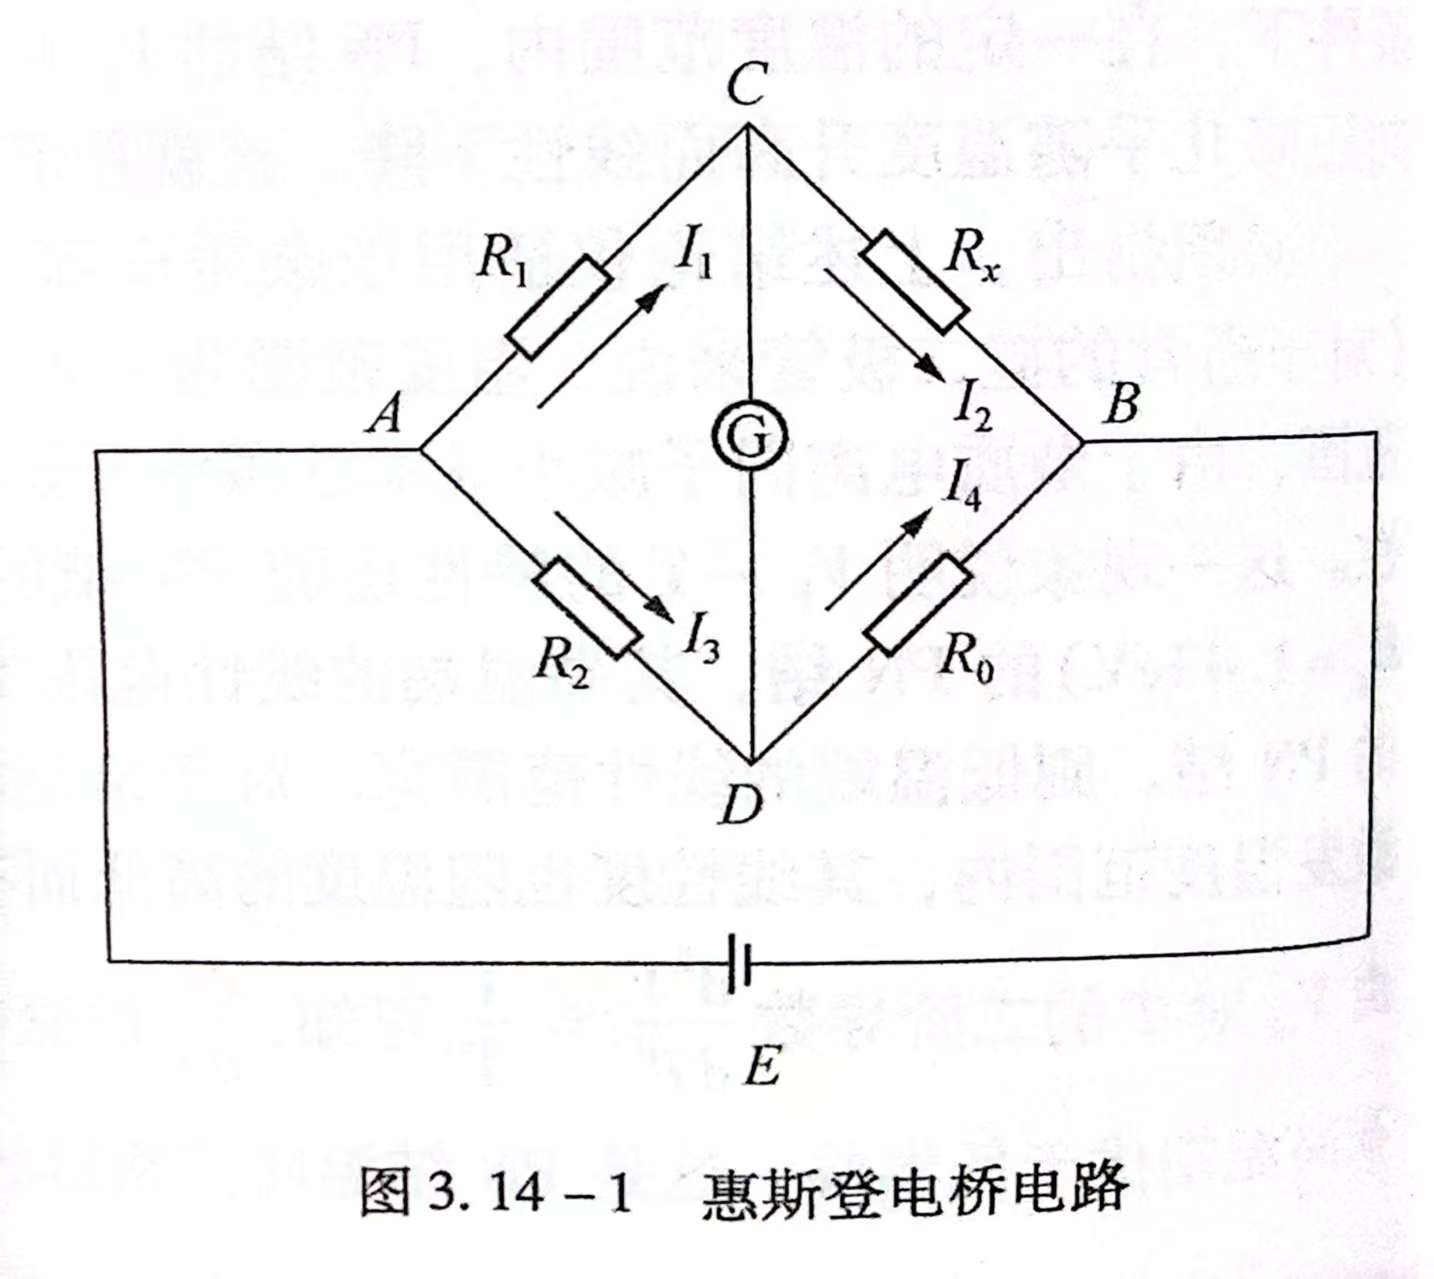
\includegraphics[width=0.5\textwidth]{assets/Wheatstonebridge.jpg}
			\caption{惠斯登电桥电路}
		\end{figure}
		
	\end{frame}

	\begin{frame}
		\frametitle{惠斯登电桥的平衡条件}
		
		当$C$和$D$两点电位相等时（即$V_{AC} = V_{AD}$），检流计中无电流通过，电桥达到平衡，此时：
		
		\begin{align}
			\frac{R_1}{R_x} = \frac{R_2}{R_0}
		\end{align}
		
		即：
		
		\begin{align}
			R_x = \frac{R_1}{R_2}R_0 = KR_0
		\end{align}
		
		式中，$K = \frac{R_1}{R_2}$称为比率。若$R_1$、$R_2$、$R_0$（或$K$和$R_0$）为已知，$R_x$即可由上式求出。
		
	\end{frame}

	\begin{frame}
		\frametitle{电桥的灵敏度}
		
		公式$R_x = \frac{R_1}{R_2}R_0 = KR_0$是在电桥平衡条件下的结果，而电桥是否平衡，实际上是通过检流计有无偏转来判断的。
		
		\begin{itemize}
			\item 检流计的灵敏度总是有限的
			\item 实验室所用的检流计，指针偏转1格所对应的电流大约为$10^{-6}$ A
			\item 当通过它的电流比$10^{-7}$还要小时，指针的偏转小于0.1格，很难观察出来
			\item 数字检流计可检测到$10^{-8}$ A级别的电流
		\end{itemize}
		
	\end{frame}
     
	\begin{frame}
		\frametitle{电桥灵敏度的定义}
		
		电桥灵敏度$S$的概念定义为：
		
		\begin{align}
			S = \frac{\Delta n}{\Delta R_x/R_x}
		\end{align}
		
		式中，$\Delta R_x$是在电桥平衡后$R_x$的微小改变量（实际上待测电阻$R_x$是不变的，改变的是电阻$R_0$）；$\Delta n$是由于电桥偏离平衡而引起的检流计指针偏转的格数。
		
		$S$越大，说明电桥越灵敏，误差也就越小。
		
		在实际中，通常$R_0$是可变的，因此：
		
		\begin{align}
			S = \frac{\Delta n}{\Delta R_0/R_0}
		\end{align}
		
	\end{frame}
    \begin{frame}
		\frametitle{电压对电桥灵敏度的影响}
         
		如果由于检流计灵敏度不够,或通过它的电流太微弱而无法觉察出来，可以吧\textbf{电源电压增高，从而使微弱电流相应增大}

		可以证明电桥灵敏度普遍表达式为:
		$$
		S=\frac{S_1E}{(R_1+R_2+R_3+R_x)+(2+\frac{R_2}{R_1}+\frac{R_x}{R_0})R_G}
		$$

		其中$S_1=\frac{\Delta n}{\Delta I_G}$为检流计敏感度。
	\end{frame}
	\begin{frame}
		\frametitle{电桥的测量误差估算}
		
		当在符合仪器规定的参考条件下使用时，根据JJQ125-86文件规定，电桥的基本误差极限可用下式表示：
		
		\begin{align}
			E_{lim} = \pm\frac{\alpha}{100}(\frac{R_n}{10} + R_0)k
		\end{align}
		
		式中，$\alpha$为电桥的准确度等级；$k$为缩放因子，取电桥的比率；$R_0$为测量盘示值；$R_n$为基准值，各有效量程的基准值应为该量程内最大值的10的整数幂。
		
	\end{frame}

	\begin{frame}
		\frametitle{电桥实验误差的估测}
		
		一般在实验中由电桥的灵敏度引入的误差$\Delta R$是这样估测的：
		
		在电桥平衡时，将$R_0$改变$\Delta R_0$，使检流计指针偏转的格数$\Delta n = 2$，而人的眼睛观察到的界限是0.2格，所以取：
		
		\begin{align}
			\Delta R = 0.2 \times \frac{\Delta R_0}{2}
		\end{align}
		
		$\Delta R$反映了平衡判断中可能包含的误差。$\Delta R$越大，电桥越不灵敏。
		
		测量结果误差可表示为
		$$
		\sigma_R \approx \sqrt{E_{lim}^2+(\Delta R)^2}
		$$
	\end{frame}

	\begin{frame}
		\frametitle{交换测量法（互易法）}
		
		用交换$R_0$和$R_x$的测量法可消除因$R_1$、$R_2$引入的误差，但在保持$R_1/R_2$比值不变的条件下，将$R_0$和$R_x$交换位置，调节$R_0$为$R_0'$，使电桥重新平衡，则：
		
		\begin{align}
			R_x = \sqrt{R_0 \cdot R_0'}
		\end{align}
		
		这表明使用交换法可消除由$R_1$、$R_2$引入$R_x$的误差。
		
	\end{frame}

	\section{实验仪器}

	\begin{frame}
		\frametitle{实验仪器}
		
		\begin{itemize}
			\item 9孔插件板
			\item JK-31稳压电源
			\item 恒流源
			\item 数字万用表
			\item 电阻箱（2000$\Omega$, 1k$\Omega$, 10k$\Omega$）
			\item 检流计
			\item 连接线
		\end{itemize}
		
		\begin{figure}
			\centering
			% 图片位置：实验仪器照片
			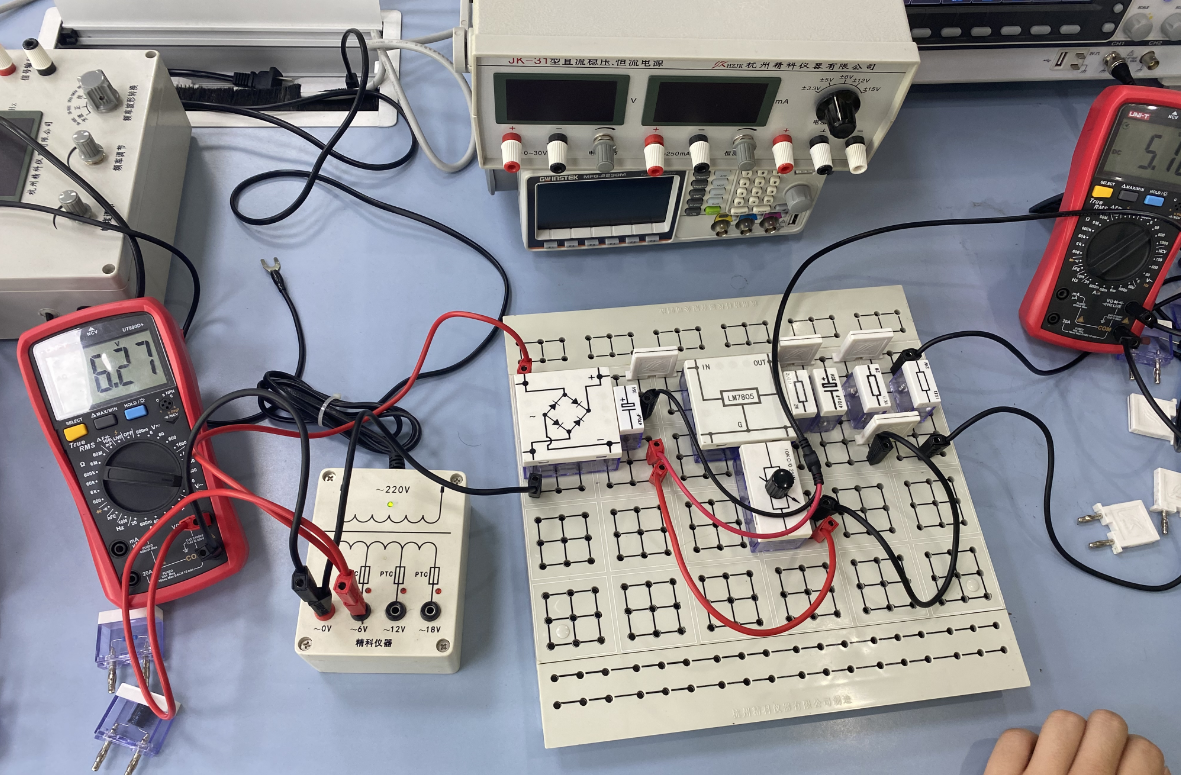
\includegraphics[width=0.6\textwidth]{assets/instruments.png}
			\caption{实验仪器}
		\end{figure}
		
	\end{frame}

	\section{实验步骤}

	\begin{frame}
		\frametitle{用自搭电桥测电阻$R_x$}
		
		\begin{enumerate}
			\item 按图连线。图中$R_M = 10\mathrm{k}\Omega$，作用是保护检流计及使平衡状态的调节；$R_0$为电阻箱；$R_x$为待测电阻；$R_1$和$R_2$为一滑线变阻器。
			
			\begin{figure}
				\centering
				% 图片位置：自搭电桥电路图
				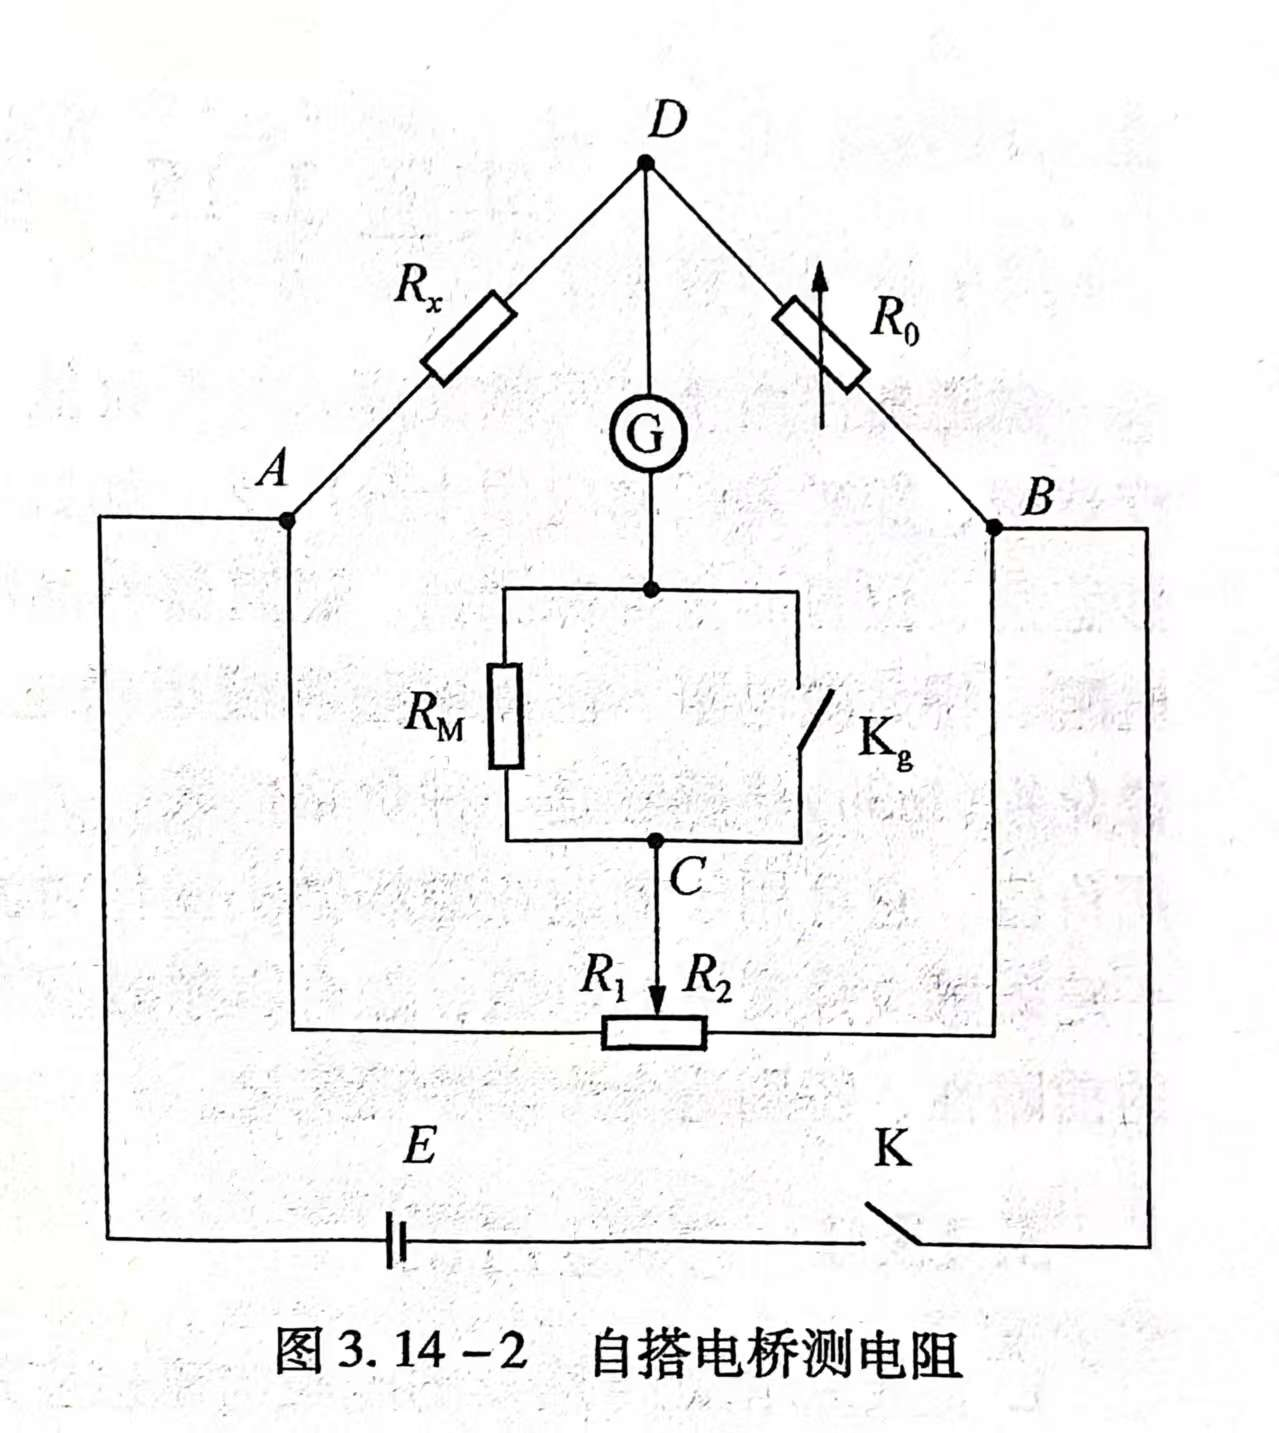
\includegraphics[width=0.5\textwidth]{assets/self_bridge.jpg}
				\caption{自搭电桥测电阻}
			\end{figure}
		\end{enumerate}
		
	\end{frame}

	\section{实验步骤与数据记录处理}

	\begin{frame}
		\frametitle{方法一：万用表直接测量电阻}
		
		\begin{columns}
			\begin{column}{0.55\textwidth}
				\begin{enumerate}
					\item 用万用表直接测量电阻$R_{x1}$、$R_{x2}$、$R_{x3}$的阻值
					\item 记录读数作为参考标准值
					\item 注意选择合适的量程，确保测量精度
				\end{enumerate}
				
				\vspace{0.5cm}
				\begin{table}
					\centering
					\begin{tabular}{|c|c|}
						\hline
						被测电阻 & 万用表测量电阻 \\
						\hline
						$R_{x1}$ & $R_{x1}=$ \\
						\hline
						$R_{x2}$ & $R_{x2}=$ \\
						\hline
						$R_{x3}$ & $R_{x3}=$ \\
						\hline
					\end{tabular}
					\caption{万用表测量数据记录}
				\end{table}
			\end{column}
			
			\begin{column}{0.45\textwidth}
				\begin{figure}
					\centering
					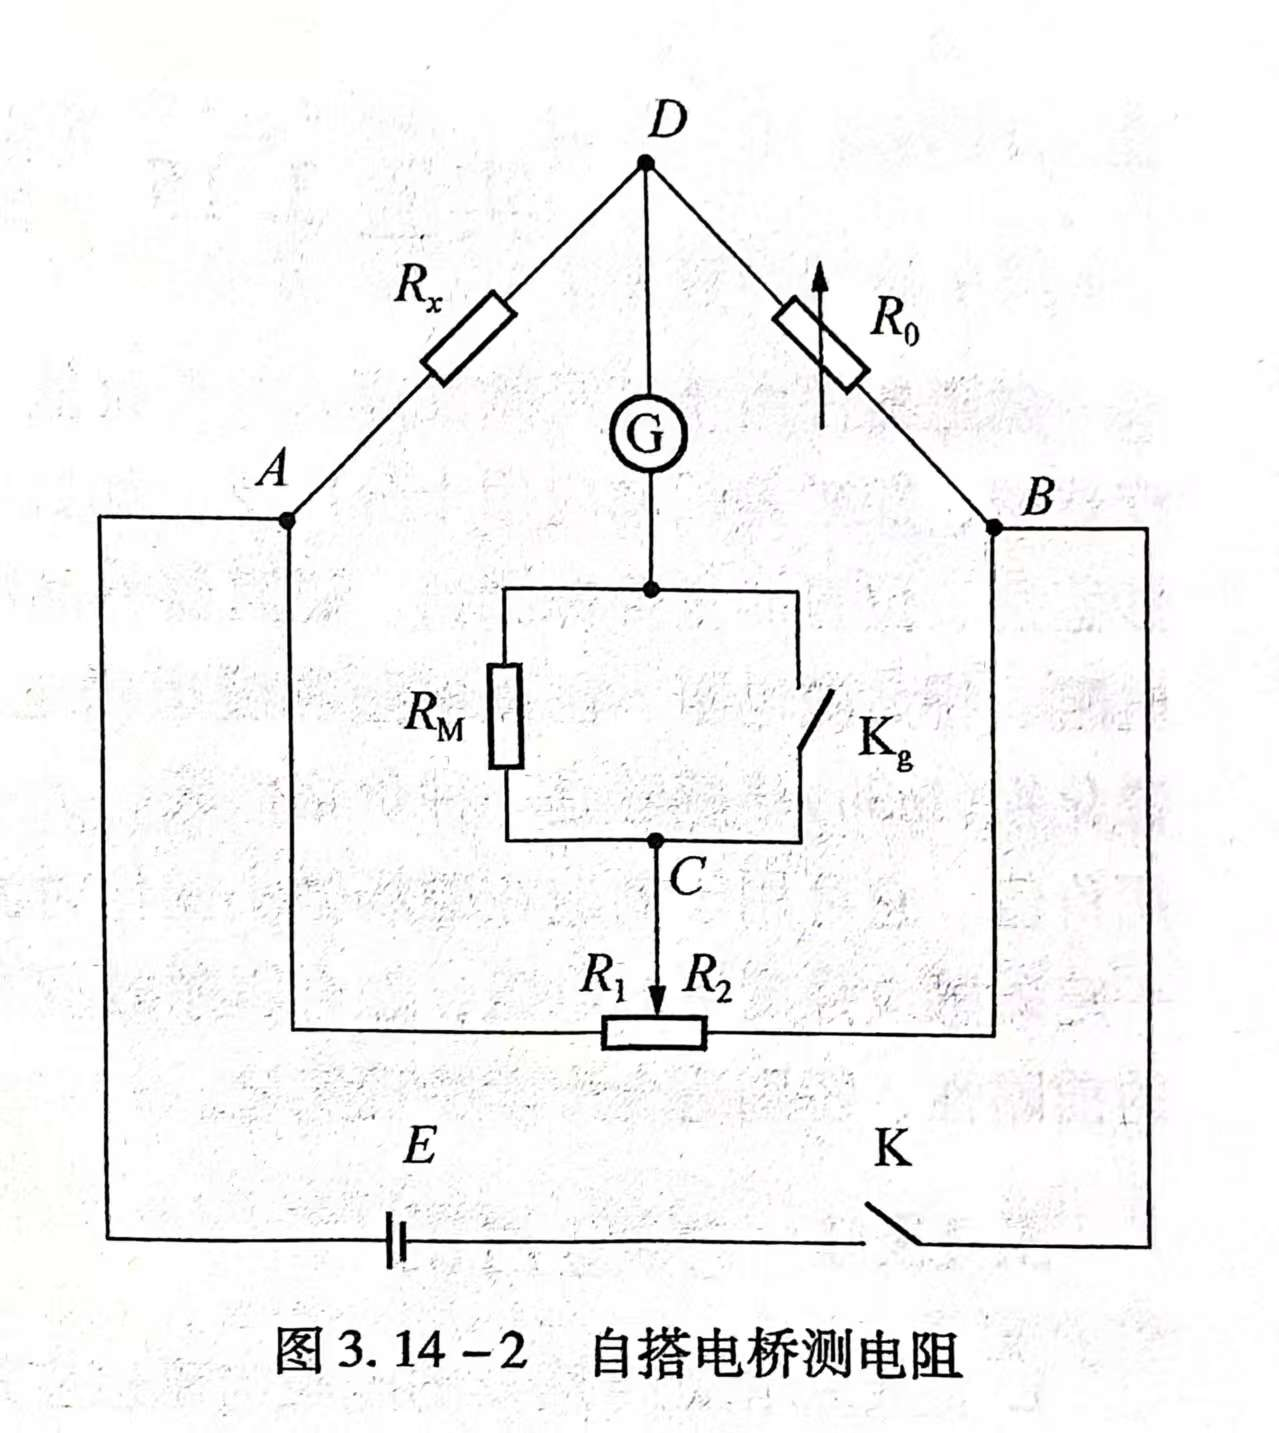
\includegraphics[width=\textwidth]{assets/self_bridge.jpg}
					\caption{自搭电桥电路图}
				\end{figure}
			\end{column}
		\end{columns}
	\end{frame}
	
	\begin{frame}
		\frametitle{方法二：惠斯登电桥测量电阻}
		
		\begin{columns}
			\begin{column}{0.5\textwidth}
				\begin{enumerate}
					\item 按图连接电路，$R_M = 10\mathrm{k}\Omega$
					\item 设置电源电压$E = 5\mathrm{V}$
					\item 调节$R_0$使电桥平衡（检流计无电流）
					\item 调节$R_0$使检流计指示为$+0.1\mu\mathrm{A}$，记录$R_0$值
					\item 调节$R_0$使检流计指示为$-0.1\mu\mathrm{A}$，记录$R_0$值
					\item 记录使检流计偏转$\pm2$格时的$\Delta R_0$值
					\item 根据公式$R_x = \frac{R_1}{R_2}R_0 = KR_0$计算$R_x$
				\end{enumerate}
			\end{column}
			
			\begin{column}{0.5\textwidth}
				\begin{figure}
					\centering
					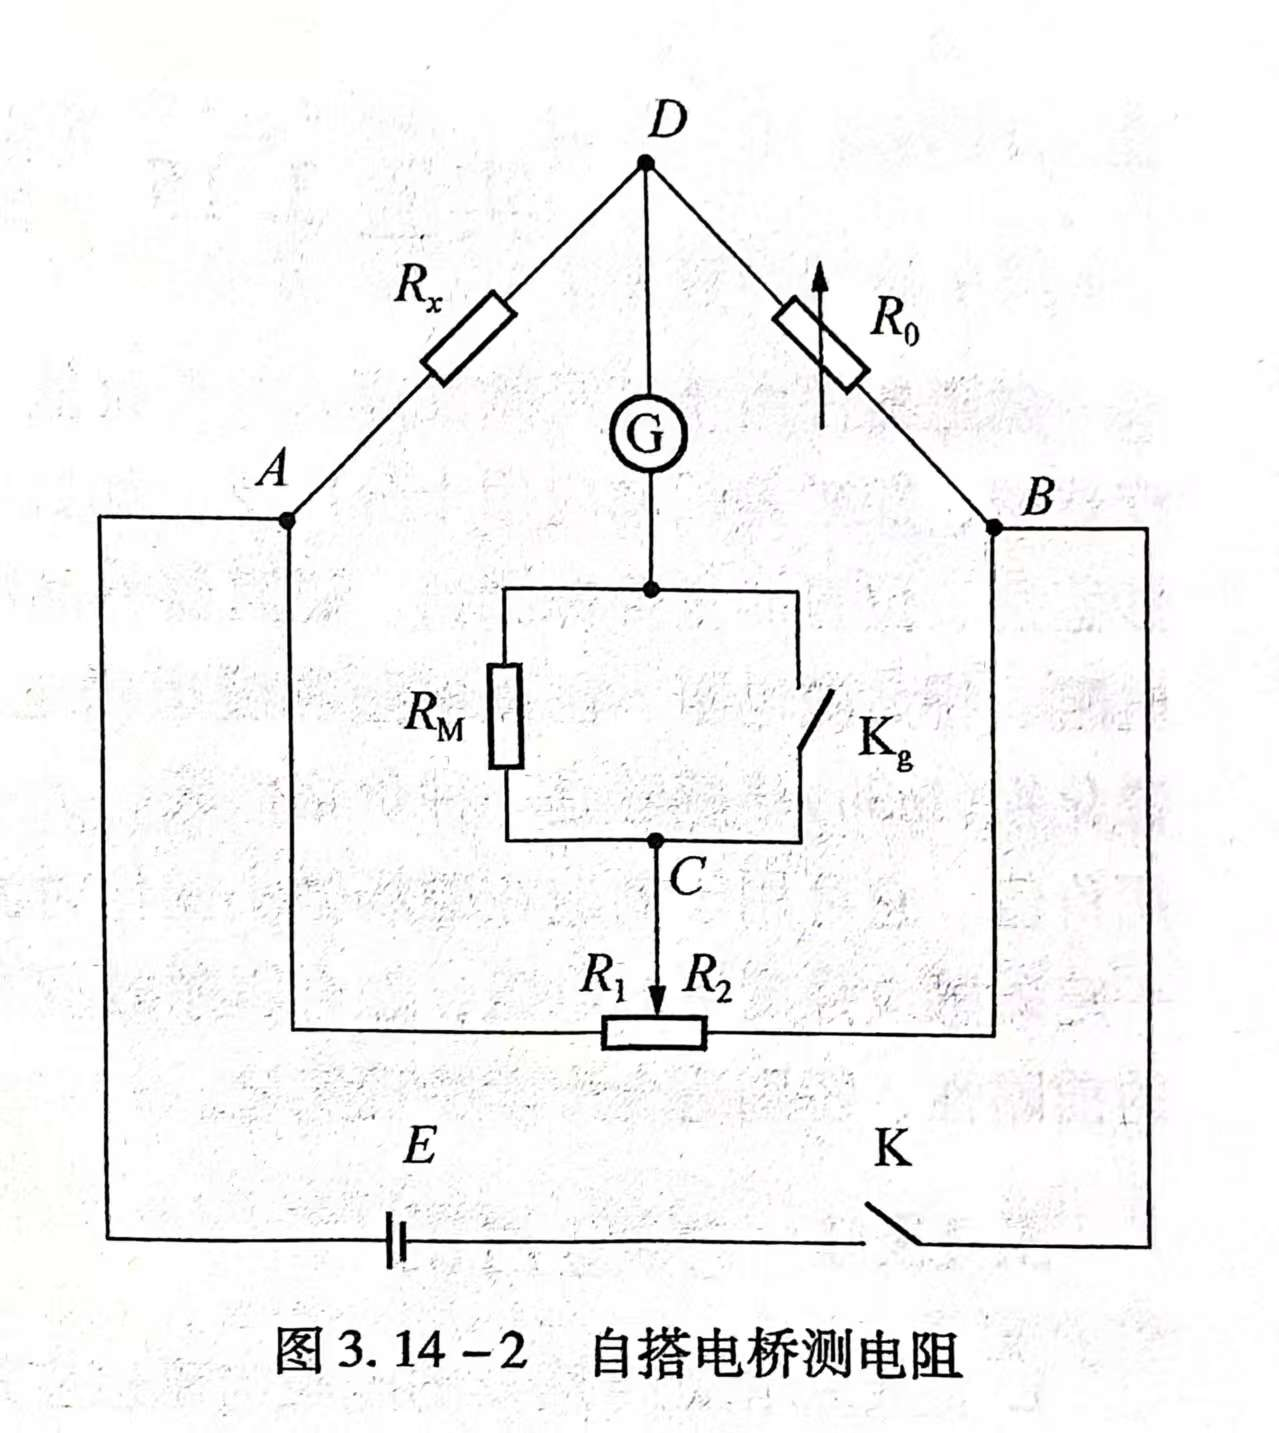
\includegraphics[width=0.5\textwidth]{assets/self_bridge.jpg}
					\caption{自搭电桥电路图}
				\end{figure}
				
				\vspace{0.3cm}
				\begin{table}
					\scriptsize
					\centering
					\begin{tabular}{|c|c|c|c|c|}
						\hline
						\multirow{3}{*}{被测电阻} & \multicolumn{4}{c|}{惠斯登电桥测量电阻} \\
						\cline{2-5}
						& \multicolumn{2}{c|}{$R_0=$} & & \\
						\cline{2-5}
						& $+0.1\mu\mathrm{A}$ & $-0.1\mu\mathrm{A}$ & & \\
						\cline{2-5}
						& $+\Delta R_0=$ & $-\Delta R_0=$ & & \\
						\hline
					\end{tabular}
					\caption{惠斯登电桥测量数据记录}
				\end{table}
			\end{column}
		\end{columns}
	\end{frame}
	
	\begin{frame}
		\frametitle{方法三：互易法测量电阻}
		
		\begin{columns}
			\begin{column}{0.4\textwidth}
				\begin{enumerate}
					\item 保持电路和比率臂$R_1/R_2$不变
					\item 记录电桥平衡时$R_S$（与$R_0$位置相同）
					\item 交换$R_0$与$R_x$位置，重新调节电桥平衡
					\item 调节以获得$\pm0.1\mu\mathrm{A}$时的$R_S'$值
					\item 记录使检流计偏转$\pm2$格时的$\Delta R_0$值
					\item 根据公式$R_x = \sqrt{R_0 \cdot R_S'}$计算$R_x$
					\item 此方法可消除因$R_1$、$R_2$不准确引入的系统误差
				\end{enumerate}
			\end{column}
			
			\begin{column}{0.5\textwidth}
				\begin{figure}
					\centering
					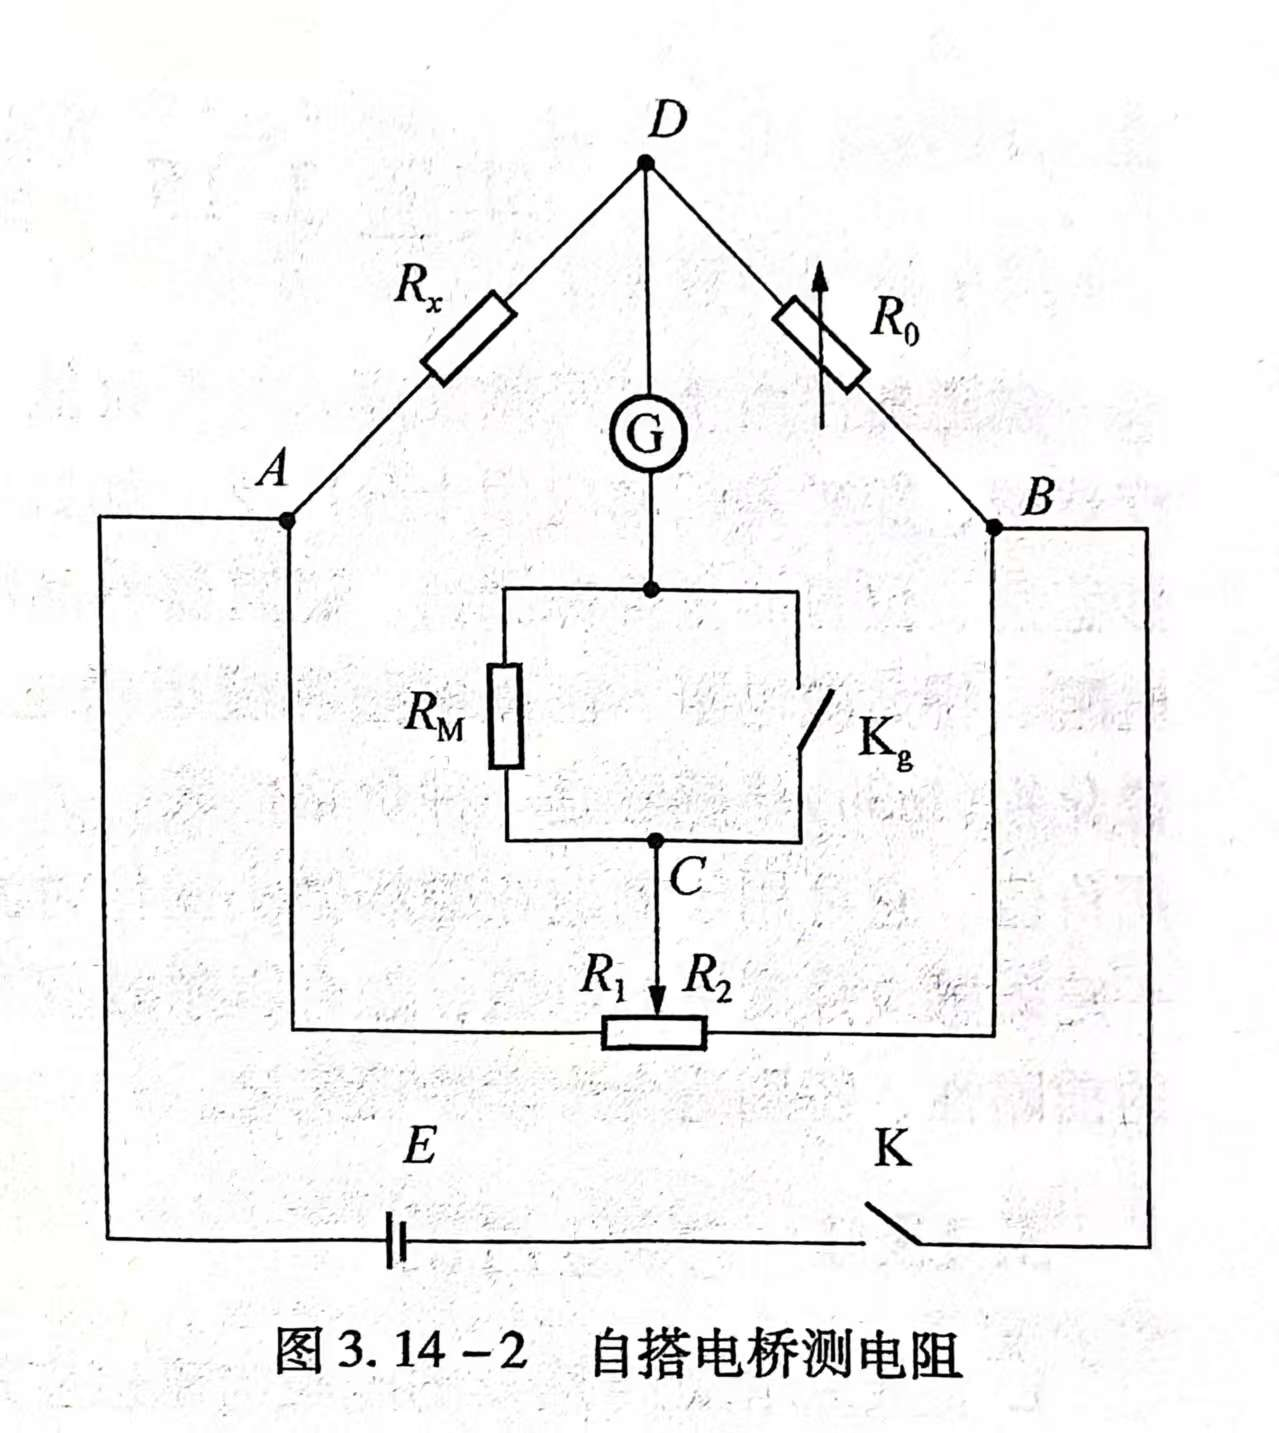
\includegraphics[width=0.5\textwidth]{assets/self_bridge.jpg}
					\caption{自搭电桥电路图}
				\end{figure}
				
				\vspace{0.1cm}
				\begin{table}
					\centering
					\resizebox{\columnwidth}{!}{
						\begin{tabular}{|c|c|c|c|c|}
							\hline
							被测电阻 & \multicolumn{2}{c|}{互易法测量电阻} & \multicolumn{2}{c|}{} \\
							\cline{2-5}
							& $R_S=$ 同 $R_0$ & & $R_S'=$ & \\
							\cline{2-5}
							\multirow{2}{*}{$R_{x1}$} & $+0.1\mu\mathrm{A}$ & $-0.1\mu\mathrm{A}$ & $+0.1\mu\mathrm{A}$ & $-0.1\mu\mathrm{A}$ \\
							\cline{2-5}
							& $+\Delta R_0=$ & $-\Delta R_0=$ & $+\Delta R_0=$ & $-\Delta R_0=$ \\
							\hline
						\end{tabular}
					}
				\end{table}
			\end{column}
		\end{columns}
	\end{frame}

	\section{注意事项}

	\begin{frame}
		\frametitle{注意事项}
		
		\begin{enumerate}
			\item 电路连接时要注意正确连接，特别是检流计的正负极性
			\item 当电桥接近平衡时，应缓慢调节$R_0$，以获得精确的平衡点
			\item 检流计的灵敏度有限，需要仔细观察指针的微小偏转
			\item 电桥平衡判断的准确性直接影响测量结果
			\item 若电流过大可能会损坏检流计，实验过程中应小心操作
			\item 交换法测量时，需保持$R_1/R_2$比值不变
		\end{enumerate}
		
	\end{frame}

	\section{误差分析}

	\begin{frame}
		\frametitle{分析一：万用表直接测量电阻的误差分析}
		
		\begin{columns}
			\begin{column}{1\textwidth}
				数字万用表测量电阻的误差分析：
				\begin{enumerate}
					\item \textbf{误差来源}：仪器本身精度限制
					\item \textbf{误差表达式}：对数字万用表，通常表示为
						\begin{align}
							\Delta R = \pm(\text{精度百分比} \times \text{读数})
						\end{align}
					\item \textbf{相对误差}：$\frac{\Delta R}{R} \times 100\%$
				\end{enumerate}
				
				\begin{alertblock}{误差计算}
					例如：万用表测得$R_{x1} = 470\Omega$，精度为$\pm 0.5\%$
					
					则绝对误差：$\Delta R = \pm 0.5\% \times 470\Omega = \pm 2.35\Omega$
					
					相对误差：$\frac{\Delta R}{R} \times 100\% = \frac{2.35}{470} \times 100\% = 0.5\%$
				\end{alertblock}
			\end{column}
		\end{columns}
	\end{frame}
	
	\begin{frame}
		\frametitle{分析二：惠斯登电桥测量电阻的误差分析}
		
		\tiny % 减小整个幻灯片的字体大小
		\setlength{\itemsep}{0pt} % 减小条目间距
		\setlength{\abovedisplayskip}{2pt} % 减小公式上方间距
		\setlength{\belowdisplayskip}{2pt} % 减小公式下方间距
		
		惠斯登电桥测量的误差主要来源于两部分：
		
		\begin{enumerate}
			\item \textbf{电桥基本误差}：根据JJQ125-86文件规定
			\begin{align}
				E_{lim} = \pm\frac{\alpha}{100}\left(\frac{R_n}{10} + R_0\right)k
			\end{align}
			其中，$\alpha$为电桥的准确度等级；$k$为比率；$R_0$为测量盘示值；$R_n$为基准值
			
			\item \textbf{平衡判断的误差}：由电桥灵敏度有限引起
			\begin{align}
				\Delta R = 0.2 \times \frac{\Delta R_0}{2}
			\end{align}
			
			检流计敏感度为$10^{-6}\mathrm{A/}$格，人眼可察觉$0.2$格偏转，$\Delta R_0$是使检流计偏转$\pm2$格的电阻变化量
		
			\item \textbf{测量结果总误差}可表示为：
			\begin{align}
				\sigma_R \approx \sqrt{E_{lim}^2+(\Delta R)^2}
			\end{align}
		\end{enumerate}
		
		\begin{alertblock}{误差计算示例}
			\scriptsize % 进一步缩小示例部分的字体
			若$R_0 = 500\Omega$，$\alpha = 0.2$，$k = 1$，$R_n = 10k\Omega$，偏转$\pm1$格时$\Delta R_0 = 5\Omega$
			
			则$E_{lim} = \pm\frac{0.2}{100}(\frac{10000}{10} + 500) \times 1 = \pm3\Omega$
			
			$\Delta R = 0.2 \times \frac{5}{2} = 0.5\Omega$
			
			总误差$\sigma_R \approx \sqrt{3^2+0.5^2} = \sqrt{9.25} \approx 3.04\Omega$
			
			相对误差：$\frac{\sigma_R}{R_x} \times 100\% = \frac{3.04}{500} \times 100\% = 0.61\%$
		\end{alertblock}
	\end{frame}
	
	\begin{frame}
		\frametitle{分析三：互易法测量电阻的误差分析}
		
		\tiny % 减小整个幻灯片的字体大小
		\setlength{\itemsep}{0pt} % 减小条目间距
		\setlength{\abovedisplayskip}{2pt} % 减小公式上方间距
		\setlength{\belowdisplayskip}{2pt} % 减小公式下方间距
		
		互易法测量电阻的误差分析需考虑$R_x = \sqrt{R_0 \cdot R_0'}$中的误差传递：
		
		\begin{enumerate}
			\item 对于每次测量，类似方法二，可得$R_0$和$R_0'$的误差$\sigma_{R_0}$和$\sigma_{R_0'}$
			
			\item 根据误差传递公式，$R_x = \sqrt{R_0 \cdot R_0'}$的相对误差为：
			\begin{align}
				\frac{\sigma_{R_x}}{R_x} = \frac{1}{2}\sqrt{\left(\frac{\sigma_{R_0}}{R_0}\right)^2 + \left(\frac{\sigma_{R_0'}}{R_0'}\right)^2}
			\end{align}
			
			\item 互易法消除了因$R_1$、$R_2$不准确引入的系统误差，但仍存在随机误差，主要来自平衡判断
		\end{enumerate}
		
		\begin{alertblock}{误差计算示例}
			\scriptsize % 进一步缩小示例部分的字体
			假设$R_0 = 500\Omega$, $\sigma_{R_0} = 3\Omega$，$R_0' = 510\Omega$，$\sigma_{R_0'} = 3.1\Omega$
			
			则$R_x = \sqrt{500 \times 510} = \sqrt{255000} \approx 505\Omega$
			
			相对误差：
			\begin{align}
				\frac{\sigma_{R_x}}{R_x} &= \frac{1}{2}\sqrt{\left(\frac{3}{500}\right)^2 + \left(\frac{3.1}{510}\right)^2}\\
				&= \frac{1}{2}\sqrt{(0.006)^2 + (0.0061)^2}\\
				&= \frac{1}{2}\sqrt{0.000073} \approx 0.0043
			\end{align}
			
			绝对误差：$\sigma_{R_x} = 0.0043 \times 505\Omega \approx 2.17\Omega$
			
			相对误差百分比：$0.0043 \times 100\% = 0.43\%$
		\end{alertblock}
		
		\footnotesize % 最后结论稍微大一点字
		互易法测量的误差明显小于方法二，体现了交换法消除系统误差的优势。
	\end{frame}

	\begin{frame}
		\frametitle{误差分析}
		
		电桥测量中的误差主要来源：
		\begin{enumerate}
			\item 仪器本身的误差
			\item 电桥灵敏度有限导致的判断误差
			\item $R_1$和$R_2$的不准确性引入的误差（可通过交换法消除）
			\item 检流计灵敏度不够或通过它的电流太微弱而无法观察出来
			\item 连接线和接触电阻的影响
			\item 温度变化对电阻值的影响
		\end{enumerate}
		
		使用交换法可以有效消除因$R_1$、$R_2$不准确引入的系统误差，提高测量精度。
		
	\end{frame}

	\section{思考题解答}

	\begin{frame}
		\frametitle{思考题解答}
		
		\small % 减小字体大小
    \setlength{\itemsep}{0pt} % 减小 enumerate 环境的行距
    
	\begin{enumerate}
        \item 试证明：自搭电桥用交换法测量$R_x$时，$R_x = \sqrt{R_0 \cdot R_0'}$
        
        \begin{proof}
            \setlength{\abovedisplayskip}{2pt} % 减小公式上方的间距
            \setlength{\belowdisplayskip}{2pt} % 减小公式下方的间距
            
            当电桥平衡时，有：
            \[
            \frac{R_x}{R_1} = \frac{R_0}{R_2} \Rightarrow \frac{R_x}{R_0} = \frac{R_1}{R_2} \quad (1)
            \]
            
            交换$R_0$和$R_x$位置后，再次平衡：
            \[
            \frac{R_0'}{R_1} = \frac{R_x}{R_2} \Rightarrow \frac{R_0'}{R_x} = \frac{R_1}{R_2} \quad (2)
            \]
            
            由(1)和(2)得：$\frac{R_x}{R_0} = \frac{R_0'}{R_x}$，交叉相乘：
            \[
            R_x^2 = R_0 R_0'
            \]
            
            因此：$R_x = \sqrt{R_0 R_0'}$。
        \end{proof}
    \end{enumerate}
		
	\end{frame}

	\begin{frame}
		\frametitle{思考题解答（续）}
		
		\begin{enumerate}\setcounter{enumi}{1}
			\item 如果没有检流计，如何用自搭电桥来测量表头内阻？
			
			可以用电压测量法：将电压表接在电桥的C、D两点间，调节$R_0$使电压表示数最小（趋近于零），此时电桥平衡。或者用数字万用表替代检流计，观察电流最小值确定平衡点。
		\end{enumerate}
		
		\begin{figure}
			\centering
			% 图片位置：无检流计测量方法示意图
			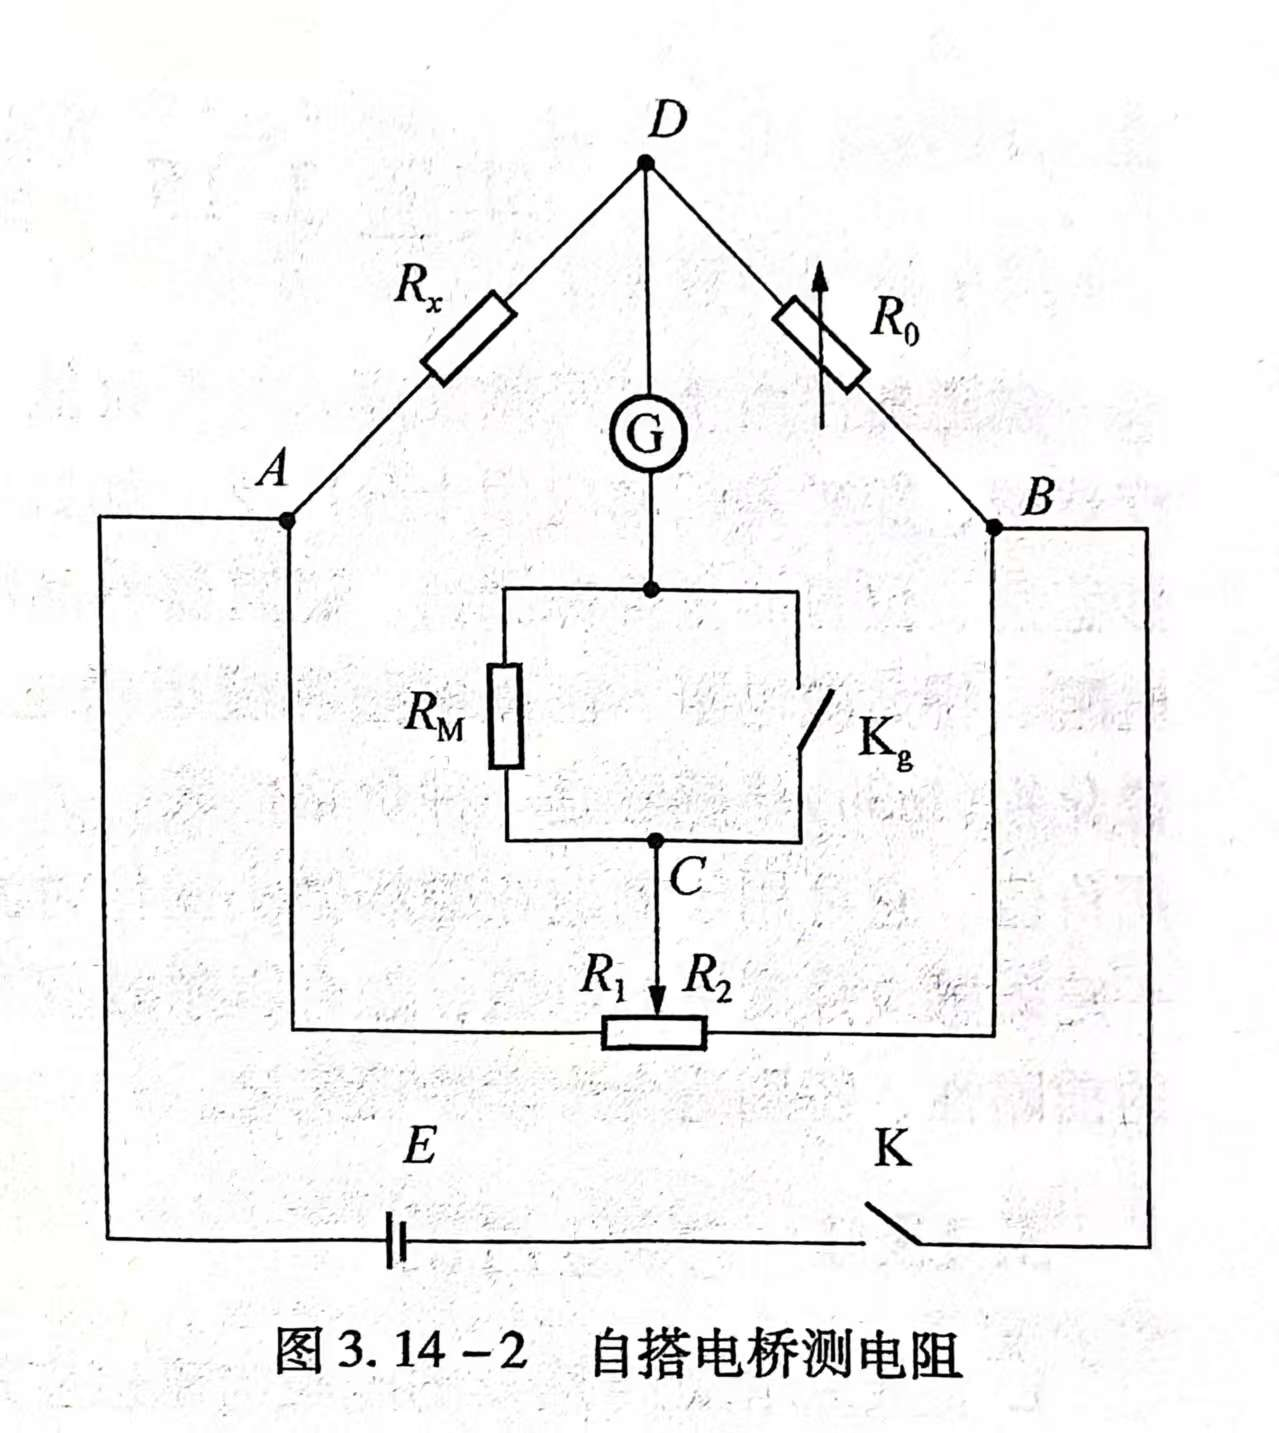
\includegraphics[width=0.43\textwidth]{assets/self_bridge.jpg}
			\caption{无检流计测量方法}
		\end{figure}
		
	\end{frame}

	% Insert a thank your frame ------------------------------------------------
	\begin{frame}
		\Huge{\centerline{Thanks!}}
	\end{frame}
	
\end{document}
